\documentclass[a4paper]{article}
\usepackage{graphicx}
\usepackage{amsmath,amssymb}
\usepackage{hyperref}
\usepackage{minted}
\usepackage{multirow}

\title{With Transformer}
\date{}
\begin{document}
    \maketitle
    This is the vanilla experiment against which we compare the results with other experiments. So it uses a single multi-head transformer on a whole event specific knowledge
    
    \section{Training}
        In this experiment we used simplest transformers.
        \begin{itemize}
            \item We considered all time steps as equal (So we are dealing with a sequence and not a time serie)
            \item No normalization or standardization is applied
            \item number of attentionheads: \textbf{8}
        \end{itemize}
        
    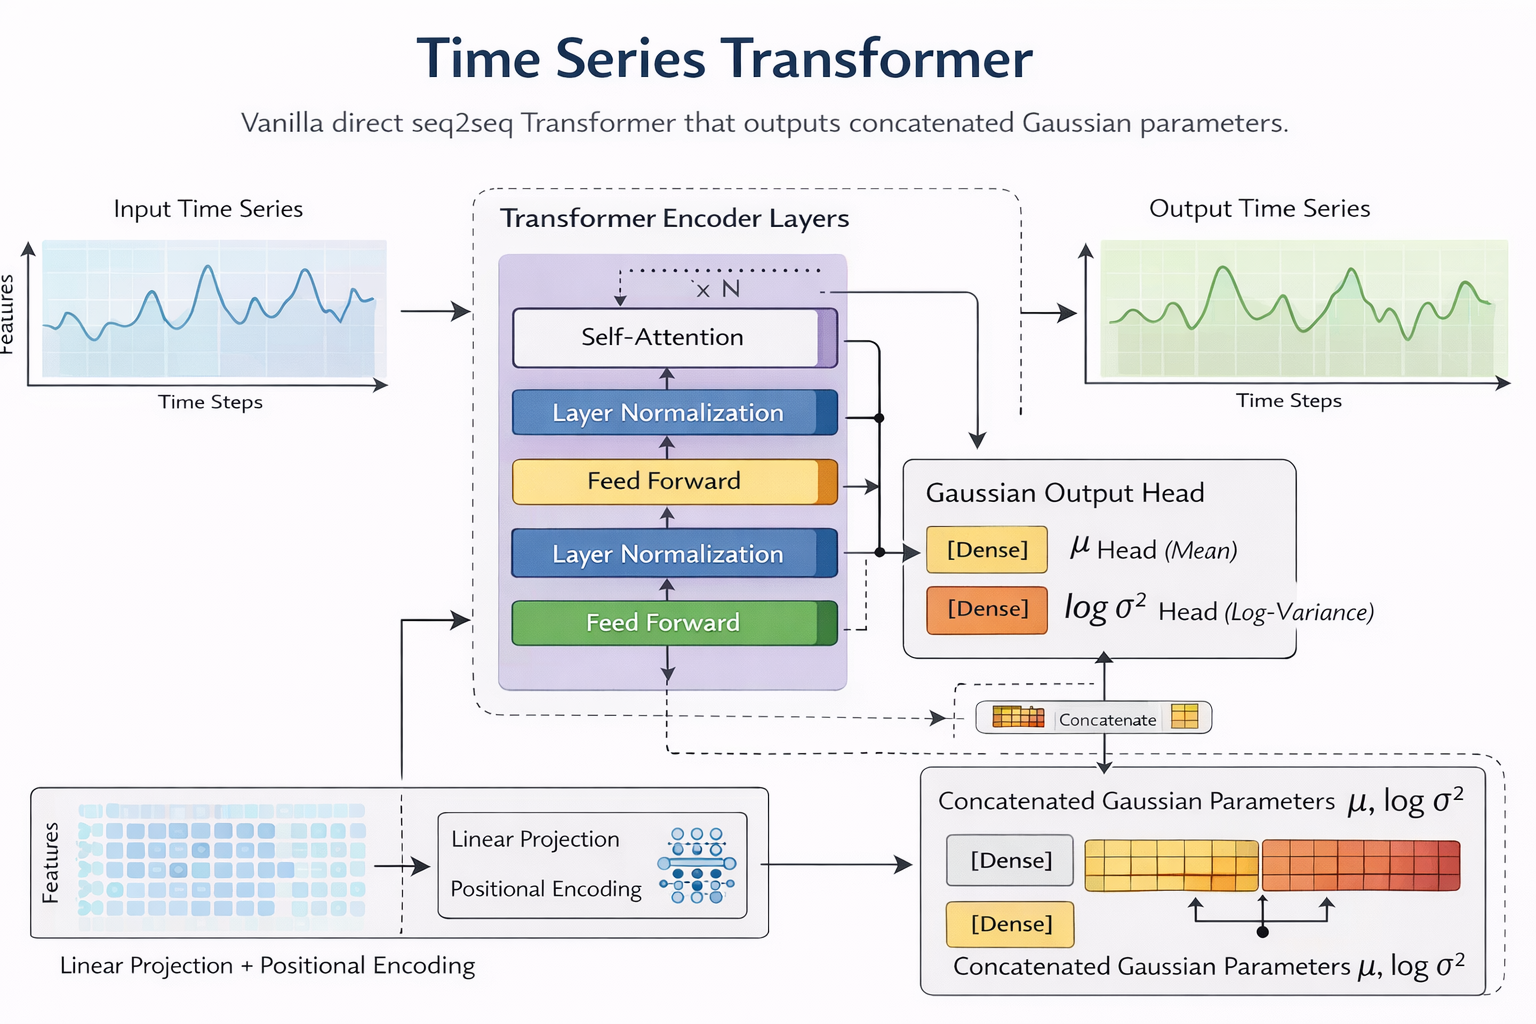
\includegraphics[scale=0.3]{transformer_architecture.png}
    
    
    \section{Results}
    
    
\end{document}